\documentclass[letterpaper,11pt]{report}

\usepackage{multirow}
\usepackage{graphicx,url}

\usepackage{ucs}
\usepackage[utf8x]{inputenc}

\setlength\topmargin{-.2in}
\setlength\oddsidemargin{-.2in}
\setlength\evensidemargin{-.2in}
\setlength\textwidth{6.9in}
\setlength\textheight{9in}

%%\usepackage[T1]{fontenc}
%%\usepackage[scaled]{helvet}
%%\renewcommand*\familydefault{\sfdefault} %% Only if the base font of the document is to be sans serif

\begin{document}

\section*{José Rafael Carrero León}

\begin{tabular}{r p{2.4in} p{46mm}}
\textbf{Dirección Actual:}&Urb. Río Aro, Villas Sta. Elena\newline
Mz. 15, No k-05 \newline
Puerto Ordaz, Edo. Bolívar & \multirow{13}{*}{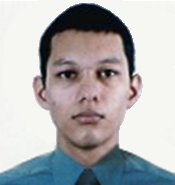
\includegraphics[scale=.8]{foto_curriculum}}\\
 & & \\
\textbf{Teléfono:}&0416 - 3105412\newline 0286 - 9520837&\\
 & & \\
\textbf{Correo Electrónico:}&josercl@gmail.com&\\
 & & \\
\textbf{Profesión:}&Ingeniero en Computación&\\
 & & \\
\textbf{Fecha de Nacimiento:}&17 de Septiembre de 1982&\\
 & & \\
\textbf{Cédula de Identidad:}&V-15.372.914&\\
 & & \\
\textbf{Idiomas:}&Espa\~{n}ol (Completo)\newline Inglés (Avanzado)&\\
\end{tabular}


\section*{Resumen}
Dominio en las instalación, configuración, administración, mantenimiento y adiestramiento de los usuarios de redes peque\~{n}as con clientes multiplataforma y servidores Linux. Dise\~{n}o y programación de soluciones Open Source centralizadas o distribuidas orientadas a la Web e integradas con bases de datos. Experiencia en la dirección de proyectos y el trabajo en equipo

\section*{Estudios Realizados}
\subsection*{Educación Profesional}
Ingeniería de Computación. Universidad Simón Bolívar. Sartenejas, Edo. Miranda.
\subsection*{Secundaria y Diversificado}
U.E. Colegio ``Loyola - Gumilla''
Ciudad Guayana, Edo. Bolívar.
\subsection*{Cadenas de Especialización Académicas}
\begin{itemize}
\item
\textbf{Principales:} Bases de Datos, Redes de Computadores, Sistemas de Información
\item
\textbf{Secundarias:} Bases de Datos en Internet, Telecomunicaciones y Economía
\end{itemize}

\section*{Habilidades Personales y Laborales}
Alta creatividad y proactividad, facilidad de análisis y resolución de problemas, fluidez comunicacional, tiempo de aprendizaje mínimo y experiencia en la dirección de proyetos y trabajo en equipo en múltiples proyectos con ajustados tiempos de entrega.

\section*{Habilidades y Conocimientos Técnicos}
\begin{itemize}
\item
\textbf{Dominio de Lenguajes de Especificación y Programación:} BASIC, C, Ensamblador, Haskell, HTML, Java, Javascript, jQuery, JSP, Linux Shell Script, PHP, Python (Básico), Prolog, Windows Shell Script, SQL, XML, XSL y LaTeX.
\item
\textbf{Uso de Ambientes de Trabajo (Frameworks):} Struts (1,2), Spring, CodeIgniter, Doctrine.
\item
\textbf{Experiencia con Sistemas Manejadores de Bases de Datos:} MySQL (instalación, configuración y soporte), ORACLE y PostgreSQL (administración intermedia y operación).
\item
\textbf{Dise\~{n}o asistido con Herramientas CASE:} PowerDesigner, Rational Rose, Rational Requisite Pro, Microsoft Visio y Microsoft Office.
\item
\textbf{Administración de Servidores:} Apache, Servidores de aplicaciones Java (Tomcat, JBoss), NFS (Network File System), NIS (Network Information Service), DNS (Domain Name Service), Firewalls (iptables).
\item
\textbf{Instalación, administración, configuración y soporte de redes:} Intranets y extranets peque\~{n}as con sistemas operativos Microsoft Windows (estaciones de trabajo) y Linux (Servidores y estaciones de trabajo).
\item
\textbf{Desarrollo de sistemas con estándares como:} UML, RUP y J2EE.
\item
\textbf{Sistemas de Control de Versiones:} Subversion, Git.
\end{itemize}

\section*{Asistencia a Congresos}
\begin{itemize}
\item
\textbf{2da. Jornada de Ingeniería Informática, Tecnología con Sentido Social.} Universidad Católica Andrés Bello. Ciudad Guayana. Junio 2009.
\item
\textbf{Foro de Desarrollo Web}. Universidad Simón Bolívar. Sartenejas, 1 y 2 de Marzo de 2004.
\item
\textbf{Taller de Inducción del Sistema de Información de Actividades de Investigación (SINAI)}. Universidad Simón Bolívar. Sartenejas, 3 de Agosto de 2003.
\item
\textbf{Olimpiadas Nacionales de Matemáticas.} Finalista. Julio 1999
\end{itemize}

\section*{Cursos Realizados}
\begin{itemize}
\item \textbf{Linux: Sistema Operativo, Comandos y Utilidad}. Servicio Nacional de Aprendizaje SENA. Noviembre 2009
\end{itemize}

\section*{Conferencias Realizadas}
\begin{itemize}
\item
\textbf{``Open Source - Linux - Instalación - Configuración - Mantenimiento''} en el Taller Nacional de Inducción al Sistema de Información de Actividades de Investigación (SINAI). Universidad Simón Bolívar, 31 Julio y 1 de Agosto de 2003.
\end{itemize}

\newpage
\section*{Experiencia Laboral}

\subsection*{Desarrollador - ESEPRIN C.A.}
  \begin{itemize}
    \item Desarrollo e implementación del Sistema de Ejecución de Manufactura (MES) -2011
        \begin{itemize}
        \item Sistema desarrollado en PHP, haciendo uso del patrón MVC
        \item Diseño de base de datos en PostgreSQL
        \item Implementación de un cliente OPC en Python para obtener información en tiempo real
        \item Diseño e implementación de programa de análisis del estado de la línea de producción basado en reglas lógicas y valores de variables en tiempo real
        \end{itemize}
    \item Instalación y Configuración de Servicios -2011
        \begin{itemize}
        \item Instalación de sistema operativo de la máquina de desarrollo (Debian Squeeze) y pruebas (Archlinux)
        \item Instalación de entorno de desarrollo Linux/Apache/Postgresql/PHP
        \item Instalación de servidor de control de versiones de Planos (Subversion)
        \item Instalación de servidor de control de versiones de código fuente (Git)
        \end{itemize}
  \end{itemize}


\subsection*{Desarrollador \emph{Freelance}}
\begin{itemize}
\item Migración del Sistema para Recursos Humanos de la Dirección Ejecutiva de la Magistratura - Octubre 2010
	\begin{itemize}
	\item Migración de la tecnología usada en el sistema de Active Server Pages (ASP) a Java
	\item La nueva versión fue desarrollada en Java 1.6 bajo la plataforma Struts 2
	\item Base de datos implementada en Oracle 10g
	\end{itemize}
\item Desarrollo e Implementación del sitio web \url{http://www.musicasacra.com.ve} - Octubre 2010
	\begin{itemize}
		\item Sitio desarrollado en PHP y MySQL, usando el ambiente de trabajo MVC Codeigniter
		\item Los aspectos de interfaz fueron desarrollados en CSS, HTML y jQuery
	\end{itemize}
\end{itemize}

\subsection*{Analista Integral III, Consorcio Kairos IT, Julio 2009 - Diciembre 2011}

\begin{itemize}
\item Parte del equipo de desarrolladores del sistema de nómina del Grupo Principal
  \begin{itemize}
    \item Sistema desarrollado usando PHP, MSSQL Server y un ambiente de trabajo MVC desarrollado en la empresa
    \item Se implementaron consultas para la generación de reportes de gestión de nómina/personal
  \end{itemize}
\end{itemize}

\begin{itemize}
\item
  Formé parte del grupo de trabajo encargado de desarollar el Sistema de Notificaciones Legales www.notifica.net
  \begin{itemize}
  \item Sistema desarrollado usando PHP, MySQL, y el Ambiente de Trabajo MVC CodeIgniter
  \item Los aspectos del cliente fueron elaborados usando CSS, HTML y Javascript usando la librería jQuery.
  \item Se implementó la firma de correos electrónicos y documentos PDF usando openssl y Java
  \item Dise\~{n}o e implementación de la base de datos del sistema
  \end{itemize}
\item
  Encargado del desarrollo y mantenimiento del sitio web de la empresa http://www.kairosit.net.
\item Instalacion del servidor de desarrollo
  \begin{itemize}
  \item Instalación del entorno LAMP (Linux, Apache, MySQL, PHP)
  \item Configuración del firewall (iptables)
  \item Instalación y configuración del control de versiones (SVN)
  \end{itemize}
\end{itemize}

\subsection*{Analista Integral II, IST Consultores, Junio 2008 - Julio 2009}
Formé parte del grupo de trabajo de desarrollo de la intranet del Banco Central de Venezuela
	\begin{itemize}
	\item Optimizacion de consultas a la base de datos dentro del sistema
	\item Dise\~{n}o y puesta en práctica de las pruebas de stress del servidor de la intranet del BCV
	\end{itemize}

\subsection*{Jefe de la Unidad de Informática, Decanato de Investigación y Desarrollo - Universidad Simón Bolívar, Enero 2007 - Diciembre 2007}
\begin{itemize}
\item Webmaster de la unidad
\item Administrador del servidor de base de datos del decanato
\item Parte del grupo de desarrolladores de sistemas
\begin{itemize}
	\item Desarrollo del Sistema de Solicitudes de Financiamiento para trabajos de investigación.
\end{itemize}
\end{itemize}

\subsection*{Decanato de Postgrado - Universidad Simón Bolívar, Enero 2006 - Diciembre 2006}
\begin{itemize}
\item Webmaster de la unidad
\item Administrador del servidor de base de datos del decanato
\item Desarrollador de sistemas en PHP y Java (JSP, Tomcat)
\end{itemize}

\subsection*{Desarrollador de Sistemas, Decanato de Investigación y Desarrollo - Universidad Simón Bolívar, Mayo 2002 - Julio 2005}
\begin{itemize}
\item Desarrollo de la segunda versión del Sistema de Información de Actividades de Investigación (SINAI)
\begin{itemize}
	\item Migración de la información existente a la nueva base de datos del sistema
	\item Implementación de la aplicación en un entorno LAMP
\end{itemize}
\item Mantenimiento de las bases de datos del SINAI
\end{itemize}

\end{document}
